\documentclass{article}
% Chinese
% \documentclass[UTF8, nofonts, mathptmx, 12pt, onecolumn]{article}
% \usepackage{xeCJK}
% \setCJKmainfont{SimSun}
\usepackage{amsmath}
\usepackage{amsfonts}
\usepackage{amssymb}
\usepackage{wasysym}
% \usepackage{ctex}
\usepackage{graphicx}
\usepackage{float}
\usepackage{geometry}
\geometry{a4paper,scale=0.8}
\usepackage{caption}
\usepackage{subcaption}
% \newcommand{\oiint}{\mathop{{\int\!\!\!\!\!\int}\mkern-21mu \bigcirc} {}}
\newcommand*{\dif}{\mathop{}\!\mathrm{d}}
\newcommand*{\md}{\mathop{}\!\mathrm{d}}
\newcommand*{\me}{\mathrm{e}}

\usepackage{parskip}
\setlength{\parindent}{0cm}

\usepackage{bm}
\let\Oldmathbf\mathbf
\renewcommand{\mathbf}[1]{\boldsymbol{\Oldmathbf{#1}}}
\let\eqnarray\align

\renewcommand*{\arraystretch}{2}
\usepackage{units}
%\renewcommand{\frac}{\nicefrac}

\usepackage{cellspace}
\setlength{\cellspacetoplimit}{5pt}
\setlength{\cellspacebottomlimit}{5pt}

\author{Xiping Hu}
\usepackage{authblk}
\author{Xiping Hu}
\affil{https://hxp.plus/}
\title{Homework for Chapter 6}

\begin{document}
\maketitle

\begin{figure}[H]
  \centering
  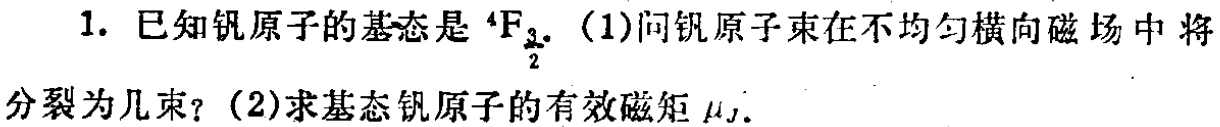
\includegraphics[width=\linewidth]{figures/Problem1}
  \label{fig:}
\end{figure}

\begin{equation*}
  \begin{aligned}
    l = 3 \quad\quad
    j = \dfrac{3}{2} \quad\quad
    s = \dfrac{3}{2} 
  \end{aligned}
\end{equation*}

$\Rightarrow$

\begin{equation*}
  \begin{aligned}
    g = 1 + \dfrac{j \left( j + 1 \right) - l \left( l + 1 \right) + s \left( s + 1 \right)}{2 j \left( j + 1 \right)} = 0.4 
  \end{aligned}
\end{equation*}

$\Rightarrow $

\begin{equation*}
  \begin{aligned}
    m = j, j - 1, \dots, -j = \dfrac{3}{2} , \dfrac{1}{2} , - \dfrac{1}{2} , - \dfrac{3}{2}   
  \end{aligned}
\end{equation*}

Since $m$ has 4 different values, the beam of atoms in magnet field will split into 4 sub-beams.

\begin{equation*}
  \begin{aligned}
    \mu_l = g \sqrt{j \left( j + 1 \right)} \mu_B = 7.18361 \times 10^{22} \  \mathrm{A \cdot m^2}
  \end{aligned}
\end{equation*}

\begin{figure}[H]
  \centering
  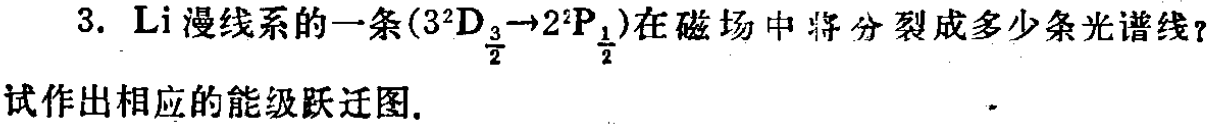
\includegraphics[width=\linewidth]{figures/Problem3}
  \label{fig:}
\end{figure}

For $3^2 D_{\frac{3}{2} }$

\begin{equation*}
  \begin{aligned}
    l = 2 \quad\quad
    j = \dfrac{3}{2} \quad\quad
    s = \dfrac{1}{2}
  \end{aligned}
\end{equation*}

$\Rightarrow $

\begin{equation*}
  \begin{aligned}
    m = j, j - 1, \dots, -j = \dfrac{3}{2} , \dfrac{1}{2} , - \dfrac{1}{2} , - \dfrac{3}{2}   
  \end{aligned}
\end{equation*}

\begin{equation*}
  \begin{aligned}
    g = 1 + \dfrac{j \left( j + 1 \right) - l \left( l + 1 \right) + s \left( s + 1 \right)}{2 j \left( j + 1 \right)} = \dfrac{4}{5} 
  \end{aligned}
\end{equation*}

For $2^2 P_{\frac{1}{2} }$

\begin{equation*}
  \begin{aligned}
    l = 1 \quad\quad
    j = \dfrac{1}{2} \quad\quad
    s = \dfrac{1}{2}
  \end{aligned}
\end{equation*}

$\Rightarrow $

\begin{equation*}
  \begin{aligned}
    m = j, j - 1, \dots, -j = \dfrac{1}{2} , - \dfrac{1}{2}   
  \end{aligned}
\end{equation*}

\begin{equation*}
  \begin{aligned}
    g = 1 + \dfrac{j \left( j + 1 \right) - l \left( l + 1 \right) + s \left( s + 1 \right)}{2 j \left( j + 1 \right)} = \dfrac{2}{3} 
  \end{aligned}
\end{equation*}

\begin{figure}[H]
  \centering
  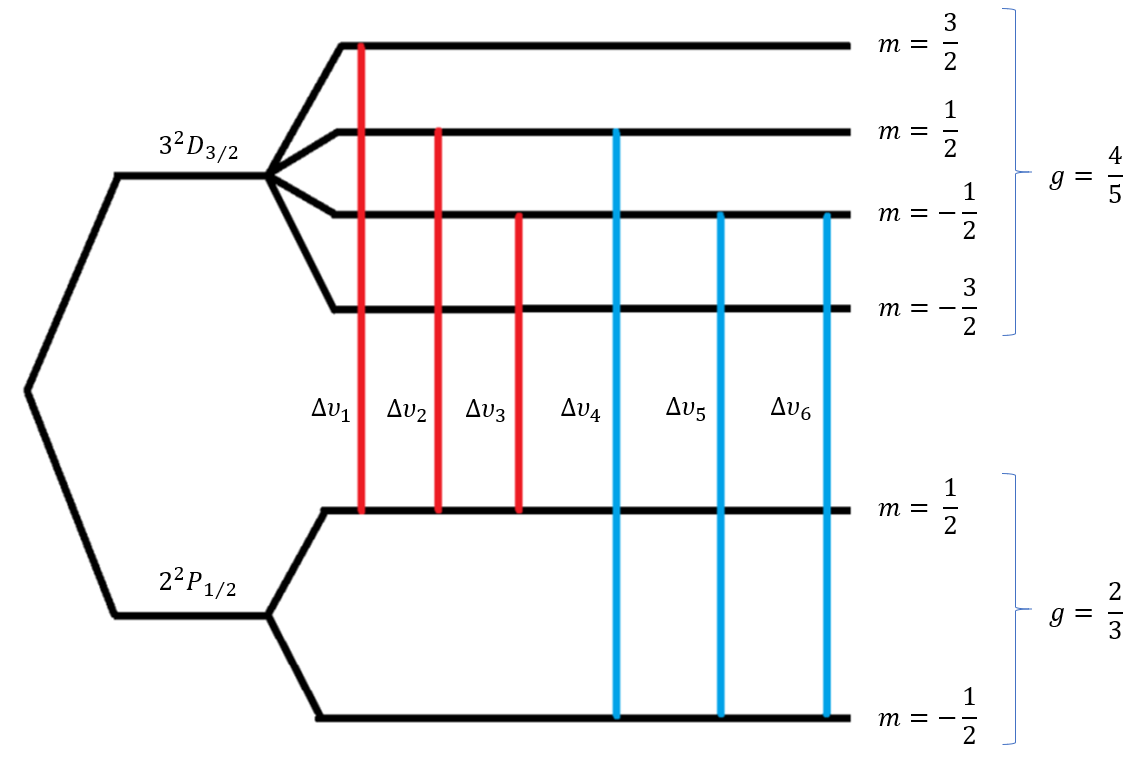
\includegraphics[width=0.9\linewidth]{figures/Problem31}
  \label{fig:}
\end{figure}

\begin{equation*}
  \begin{aligned}
    & \nu_1 = \left( \dfrac{3}{2} \cdot \dfrac{4}{5} - \dfrac{1}{2} \cdot \dfrac{2}{3} \right) L = \dfrac{13}{15} L \\    
    & \nu_2 = \left( \dfrac{1}{2} \cdot \dfrac{4}{5} - \dfrac{1}{2} \cdot \dfrac{2}{3} \right) L = \dfrac{1}{15} L \\    
    & \nu_3 = \left( - \dfrac{1}{2} \cdot \dfrac{4}{5} - \dfrac{1}{2} \cdot \dfrac{2}{3} \right) L = - \dfrac{11}{15} L \\    
    & \nu_4 = \left( \dfrac{1}{2} \cdot \dfrac{4}{5} + \dfrac{1}{2} \cdot \dfrac{2}{3} \right) L = \dfrac{11}{15} L \\    
    & \nu_5 = \left( - \dfrac{1}{2} \cdot \dfrac{4}{5} + \dfrac{1}{2} \cdot \dfrac{2}{3} \right) L = - \dfrac{1}{15} L \\    
    & \nu_6 = \left( - \dfrac{3}{2} \cdot \dfrac{4}{5} + \dfrac{1}{2} \cdot \dfrac{2}{3} \right) L = - \dfrac{13}{15} L \\    
  \end{aligned}
\end{equation*}

\begin{figure}[H]
  \centering
  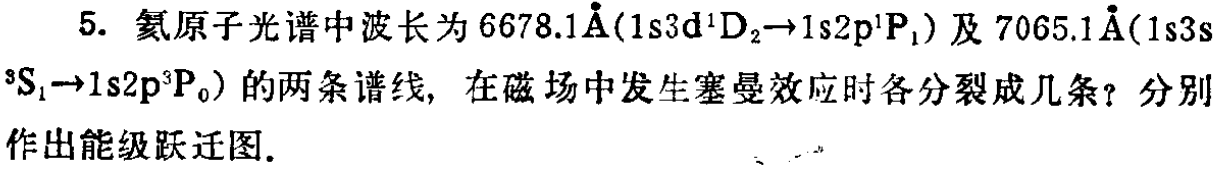
\includegraphics[width=\linewidth]{figures/Problem5}
  \label{fig:}
\end{figure}

$1s3d^1D_2 \rightarrow 1s2p^1P_1$:

\begin{equation*}
  \begin{aligned}
    & l_1 = 2 \\
    & s_1 = 0 \\
    & j_1 = 2
  \end{aligned}
  \quad\quad 
  \begin{aligned}
    & l_2 = 1 \\
    & s_2 = 0 \\
    & j_2 = 1
  \end{aligned}
\end{equation*}

\begin{equation*}
  \begin{aligned}
    g = 1 + \dfrac{j \left( j + 1 \right) - l \left( l + 1 \right) + s \left( s + 1 \right)}{2 j \left( j + 1 \right)} 
  \end{aligned}
  \Rightarrow
  \left\{
  \begin{aligned}
    & g_1 = 1 \\
    & g_2 = 1
  \end{aligned}
  \right.
\end{equation*}

\begin{equation*}
  \begin{aligned}
    m = j, j - 1, \dots, -j   
  \end{aligned}
  \Rightarrow
  \left\{
  \begin{aligned}
    & m_1 = 2,1,0,-1,-2 \\
    & m_2 = 1,0,-1
  \end{aligned}
  \right.
\end{equation*}

\begin{figure}[H]
  \centering
  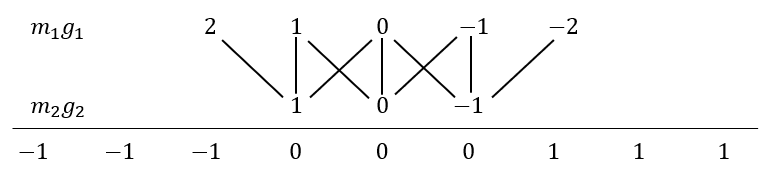
\includegraphics[width=0.6\linewidth]{figures/Problem51}
  \label{fig:}
\end{figure}

The spectral line will split into $3$ components in Zeeman effect.

$1s3s^3S_1 \rightarrow 1s2p^3P_0$:

\begin{equation*}
  \begin{aligned}
    & l_1 = 0 \\
    & s_1 = 1 \\
    & j_1 = 1
  \end{aligned}
  \quad\quad 
  \begin{aligned}
    & l_2 = 1 \\
    & s_2 = 1 \\
    & j_2 = 0
  \end{aligned}
\end{equation*}

$\Rightarrow $

\begin{equation*}
  \left\{
  \begin{aligned}
    & g_1 = 2 \\
    & g_2 = 0
  \end{aligned}
  \right.
\end{equation*}

\begin{equation*}
  \begin{aligned}
    m = j, j - 1, \dots, -j   
  \end{aligned}
  \Rightarrow
  \left\{
  \begin{aligned}
    & m_1 = 1,0,-1 \\
    & m_2 = 0
  \end{aligned}
  \right.
\end{equation*}

\begin{figure}[H]
  \centering
  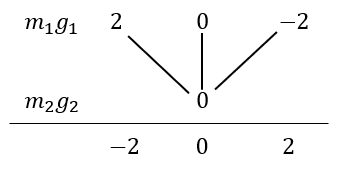
\includegraphics[width=0.25\linewidth]{figures/Problem52}
  \label{fig:}
\end{figure}

The spectral line will split into $3$ components in Zeeman effect.

\begin{figure}[H]
  \centering
  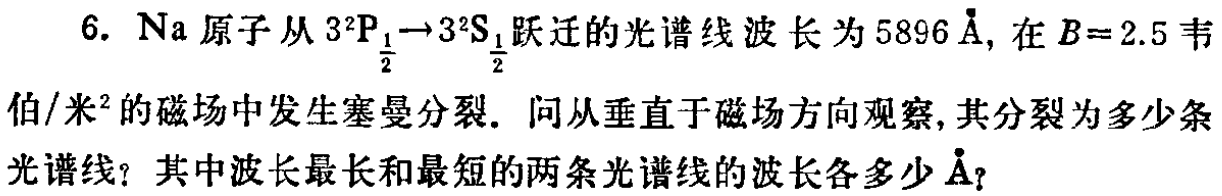
\includegraphics[width=\linewidth]{figures/Problem6}
  \label{fig:}
\end{figure}

\begin{equation*}
  \begin{aligned}
    & l_1 = 1 \\
    & s_1 = \dfrac{1}{2}  \\
    & j_1 = \dfrac{1}{2} 
  \end{aligned}
  \quad\quad 
  \begin{aligned}
    & l_2 = 0  \\
    & s_2 = \dfrac{1}{2}  \\
    & j_2 = \dfrac{1}{2} 
  \end{aligned}
\end{equation*}

$\Rightarrow $

\begin{equation*}
  \left\{
  \begin{aligned}
    & g_1 = \dfrac{2}{3}  \\
    & g_2 = 2
  \end{aligned}
  \right.
\end{equation*}

\begin{equation*}
  \begin{aligned}
    m = j, j - 1, \dots, -j   
  \end{aligned}
  \Rightarrow
  \left\{
  \begin{aligned}
    & m_1 = \dfrac{1}{2}, - \dfrac{1}{2}   \\
    & m_2 = \dfrac{1}{2}, - \dfrac{1}{2}  
  \end{aligned}
  \right.
\end{equation*}

\begin{figure}[H]
  \centering
  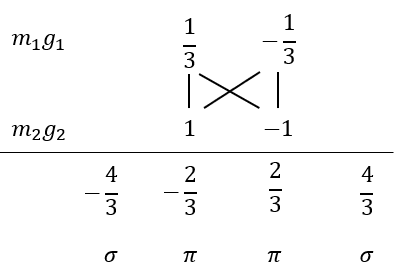
\includegraphics[width=0.4\linewidth]{figures/Problem61}
  \label{fig:}
\end{figure}

Observing in perpendicular orientation, the spectral line will split into $4$ components.

\begin{equation*}
  \begin{aligned}
    \Delta \left( \dfrac{1}{\lambda}  \right) = - \dfrac{\Delta \lambda}{\lambda^2} = \dfrac{4}{3} L \Rightarrow \Delta \lambda_{max} = \dfrac{8}{3} L \lambda^2 = 1.08 \  \text{\normalfont\AA}
  \end{aligned}
\end{equation*}

\end{document}